%% Figure from MATH 556 notes, section 44 (Lecture 19). ADDED (not from lecture).
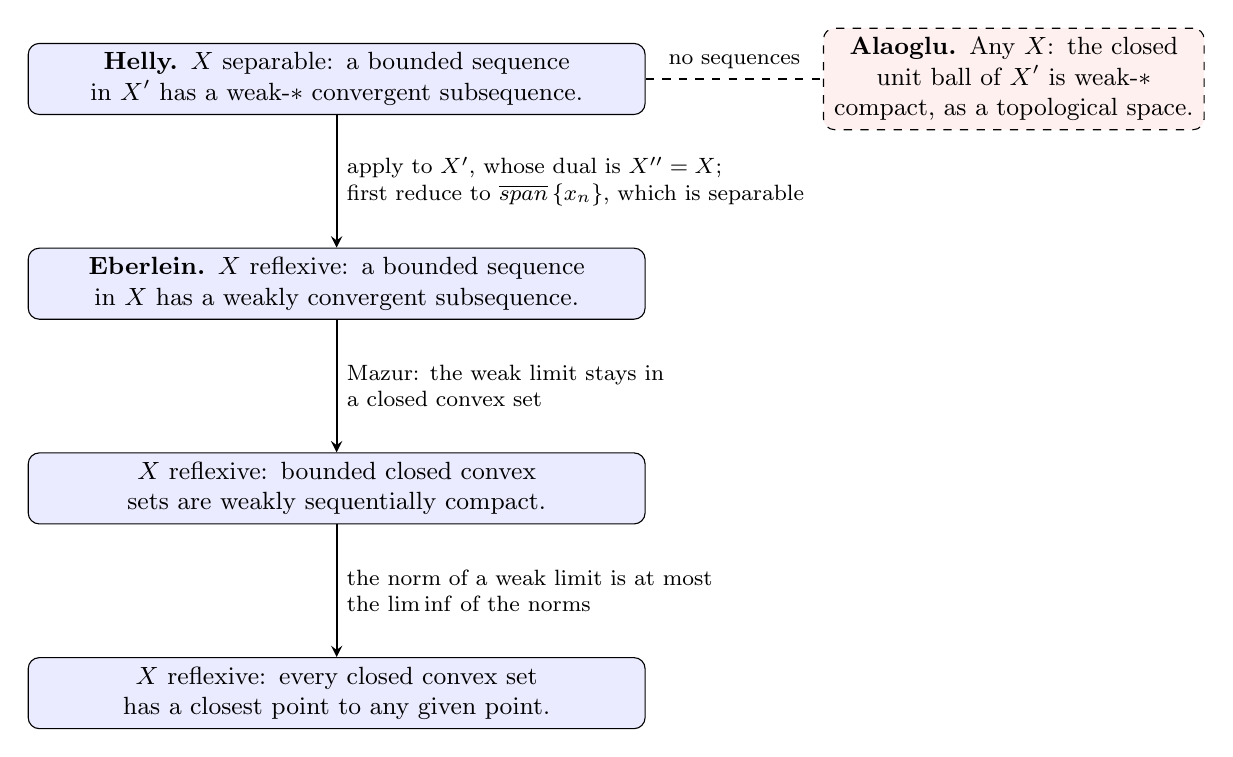
\begin{tikzpicture}[>=stealth, every node/.style={font=\small}]
  \node[draw, rounded corners, align=center, text width=7.6cm, fill=blue!8] (H) at (0,0) {\textbf{Helly.} $X$ separable: a bounded sequence in $X'$ has a weak-$*$ convergent subsequence.};
  \node[draw, rounded corners, align=center, text width=7.6cm, fill=blue!8] (E) at (0,-2.6) {\textbf{Eberlein.} $X$ reflexive: a bounded sequence in $X$ has a weakly convergent subsequence.};
  \node[draw, rounded corners, align=center, text width=7.6cm, fill=blue!8] (K) at (0,-5.2) {$X$ reflexive: bounded closed convex sets are weakly sequentially compact.};
  \node[draw, rounded corners, align=center, text width=7.6cm, fill=blue!8] (P) at (0,-7.8) {$X$ reflexive: every closed convex set has a closest point to any given point.};
  \draw[->, thick] (H) -- node[right, align=left, font=\footnotesize] {apply to $X'$, whose dual is $X'' = X$;\\ first reduce to $\overline{\operatorname{span}}\,\{x_n\}$, which is separable} (E);
  \draw[->, thick] (E) -- node[right, align=left, font=\footnotesize] {Mazur: the weak limit stays in\\ a closed convex set} (K);
  \draw[->, thick] (K) -- node[right, align=left, font=\footnotesize] {the norm of a weak limit is at most\\ the $\liminf$ of the norms} (P);
  \node[draw, dashed, rounded corners, align=center, text width=4.6cm, fill=red!6] (A) at (8.6,0) {\textbf{Alaoglu.} Any $X$: the closed unit ball of $X'$ is weak-$*$ compact, as a topological space.};
  \draw[dashed] (H) -- node[above, font=\footnotesize] {no sequences} (A);
\end{tikzpicture}
